\documentclass[runningheads]{llncs}

\usepackage{pgfplots}
\usepackage{tikz}
\usetikzlibrary{pgfplots.groupplots} % needs to be loaded exactly like this
\usepgfplotslibrary{fillbetween}
\usepgfplotslibrary{colorbrewer}
\usetikzlibrary{patterns}

\usepackage{csvsimple}
\usepackage{siunitx}
\usepackage{tabularx}
\usepackage{subcaption}
\usepackage{graphicx}
\usepackage{xargs}
\usepackage{url}
\usepackage{amssymb}
\usepackage{pifont}
\usepackage{threeparttable,tablefootnote}
\usepackage{wrapfig}
\usepackage{wasysym}
\usepackage[super]{nth}
\usepackage{listings}
\usepackage{jslistings}

\newcommand{\cmark}{\ding{51}}%
\newcommand{\xmark}{\ding{55}}%

\pgfplotsset{
    table/search path={./../../benchmark},
    every pin edge/.style={solid},
    compat=newest
}
\definecolor{cppColor}{rgb}{0,0,0}
\definecolor{nodeColor}{rgb}{0,0.6,0}
\definecolor{denoColor}{rgb}{0,0,1}
\definecolor{chromeColor}{rgb}{1,0,0}
\definecolor{firefoxColor}{rgb}{1,0.5,0}

\newcommand{\plotBenchmark}[3]{%
    \addplot+ [
        #2,
        #3,
        mark=*,
        mark options={solid,fill=#2, scale=0.5},
        error bars/.cd,
        error bar style={mark size=3pt, solid, #2},
        y dir=both,
        y explicit,
    ]
    table [
            x=sizeTheta,
            y=mean,
            y error=stdev,
            col sep=comma
        ] {#1};
}

\newenvironment{chartBenchmark}
{\begin{tikzpicture}
        \begin{axis} [
                width=\linewidth,
                height=0.45\linewidth,
                legend style={font=\tiny},
                grid,
                grid style=dashed,
                xlabel={$S_\theta$ [pixels per degree]},
                ylabel={Time [ms]},
                mark options={solid},
                legend pos=north west
            ] }
            %
            {
        \end{axis}
    \end{tikzpicture}
}

\newcommandx\groupBenchmark[6][4=1000, 5=800, 6=100]{
    \begin{tikzpicture}
        \begin{groupplot}[
                group style={
                    group size=2 by 2,
                    vertical sep=2cm
                },
                width=0.5\linewidth,
                height=0.405\linewidth,
                grid,
                grid style=dashed,
                legend style={
                        legend columns=1,
                    },
                tick label style={font=\tiny},
                every axis title shift=0pt,
                max space between ticks=20,
                ymin=0
            ]

            \nextgroupplot[
                title={SHT \textit{non-LUT}},
                ylabel={Time [ms]},
                legend to name={CommonLegend},
                xlabel={$S_\theta$ [pikseli na stopień]},
                ymax=#4
            ]
            #1

            \nextgroupplot[
                title={SHT \textit{LUT}},
                xlabel={$S_\theta$ [pikseli na stopień]},
                legend to name={CommonLegend},
                ymax=#5
            ]
            #2

            \nextgroupplot[
                title={CHT},
                xlabel={współczynnik max. promienia $n$},
                ylabel={Time [ms]},
                legend to name={CommonLegend},
                ymax=#6,
                legend cell align={left}
            ]
            #3
            
        \end{groupplot}
        \path (group c1r2.east) -- node[right, xshift=0.83cm] {\ref{CommonLegend}} (group c1r2.east);
    \end{tikzpicture}
}


\newcommand\seqReference{
    \plotBenchmark{cpp_theta_SHT_Simple.csv}{cppColor}{dashed}
    \addlegendentry{C++ Sequential};
    \plotBenchmark
    {js-sequential_theta_SHT_Simple_Firefox.csv}
    {firefoxColor}
    {name path=Firefox_Seq,opacity=0}
    \plotBenchmark
    {js-sequential_theta_SHT_Simple_Chrome.csv}
    {chromeColor}
    {name path=Chrome_Seq,opacity=0}
    \addplot [black,opacity=0.1] fill between [of=Chrome_Seq and Firefox_Seq];
}

\newcommand\seqReferenceLookup{
    \plotBenchmark{cpp_theta_SHT_Simple_Lookup.csv}{cppColor}{dashed}
    \addlegendentry{C++ Sequential};
    \plotBenchmark
    {js-sequential_theta_SHT_Simple_Lookup_Firefox.csv}
    {firefoxColor}
    {name path=Firefox_Seq_Lookup,opacity=0}
    \plotBenchmark
    {js-sequential_theta_SHT_Simple_Lookup_Chrome.csv}
    {chromeColor}
    {name path=Chrome_Seq_Lookup,opacity=0}
    \addplot [black,opacity=0.1] fill between [of=Chrome_Seq_Lookup and Firefox_Seq_Lookup];
}

\newcommand\seqReferenceCircle{
    \plotBenchmark{cpp_theta_CHT_Simple.csv}{cppColor}{dashed}
    \addlegendentry{C++ Sequential};
    \plotBenchmark
    {js-sequential_theta_CHT_Simple_Firefox.csv}
    {firefoxColor}
    {name path=Firefox_Seq,opacity=0}
    \plotBenchmark
    {js-sequential_theta_CHT_Simple_Chrome.csv}
    {chromeColor}
    {name path=Chrome_Seq,opacity=0}
    \addplot [black,opacity=0.1] fill between [of=Chrome_Seq and Firefox_Seq];
}

\newcommand{\plotColdstart}[2]{%
    \addplot+ [
        #2,
        mark=*,
        mark options={solid, scale=0.75},
        line width=0.75pt
    ]
    table [
            x=nth,
            y=time,
            col sep=comma
        ] {#1};
}


\newcommand{\plotMethod}[4]{%
    \addplot
    plot [error bars/.cd, y dir=both, y explicit]
    table [
            x=name,
            y=mean,
            y error=stdev,
            col sep=comma
        ] {methods/#1.csv};
    \pgfplotsset{cycle list shift=-#2}
    \addlegendentry{#3}
    \addplot+ [
        postaction={pattern=north east lines}
    ]
    plot [error bars/.cd, y dir=both, y explicit]  table [
            x=name,
            y=mean,
            y error=stdev,
            col sep=comma
        ] {methods/#1-lookup.csv};

    \addlegendentry{#4}
}


\begin{document}
%
\title{Performance and analysis of acceleration methods in JavaScript environments based on simplified standard Hough transform algorithm}
%
\titlerunning{Performance and analysis of acceleration methods\dots}

\author{Damian Koper \and Marek Woda}
%
% \authorrunning{D. Koper et al.}
% First names are abbreviated in the running head.
% If there are more than two authors, 'et al.' is used.
%
\institute{Faculty of Information and Communication Technology,\\
Wroclaw University of Science and Technology\\
\email{kopernickk@gmail.com, marek.woda@pwr.edu.pl}}
%
\maketitle              % typeset the header of the contribution
%
\begin{abstract}
  In this paper, we present analysis of popular acceleration methods in JavaScript execution environments including Chrome, Firefox, Node and Deno.  We focus evenly on adopting the same codebase to take advantage of every method, benchmarking our solutions and caveats of building libraries compatible with multiple environments. To compare performance, we use a simplified standard Hough transform algorithm. As a reference points of our benchmarks, we use sequential version of the algorithm written in both JavaScript and C++. Our study shows that Chrome is the fastest JS environment in every benchmark and Firefox is the slowest in which we identified optimization problems.  Overall WebGL appeared as the fastest and without parallel execution native C++ addon in Node is the most performant. We hope that this analysis will help to find the most efficient way to speed up execution making JavaScript a more robust environment for CPU-intensive computations.

  \keywords{javascript \and acceleration \and sht \and standard hough transform \and node \and browser \and deno \and webgl \and webpack \and wasm \and simd \and workers \and coldstart}
\end{abstract}

\chapter{Wstęp}

Prawo Moore'a mówi, że liczba tranzystorów w~układach scalonych podwaja się co około dwa lata. Prawo Koomey'a opisuje natomiast trend wzrostu liczby obliczeń na jeden dżul energii, która podwaja się co 1.57 lat. Choć w~ostatnich latach, w~związku ze zmniejszającym się tempem miniaturyzacji tranzystorów, wartości te przestały być aktualne to wciąż mamy do czynienia ze zjawiskiem ustawicznego wzrostu mocy obliczeniowej. Dodatkowo, zgodnie z~obserwacją nazwaną prawem Huang'a - prezesa firmy NVIDIA, wzrost wydajności układów graficznych wzrasta więcej niż dwukrotnie co dwa lata\cite{tongo}, co świadczy o~obecnym rozwoju możliwości optymalizacji architektur i~programów wykorzystujących przetwarzanie masowo równoległe.  Wzrost wydajności z~kolei zwiększa możliwości wykorzystania algorytmów, które wcześniej były zbyt intensywne obliczeniowo i~nie mogły być wykorzystane w~rozwiązaniach produkcyjnych. Powszechnie dostępne wydajne maszyny dają również możliwości szybszego prototypowania rozwiązań większej liczbie osób, co z~kolei wpływa na rozwój samych algorytmów i~ich zastosowań. Algorytmy i~obliczenia opierają się na osiągnięciach analizy numerycznej oraz matematyki dyskretnej.

Analiza numeryczna zajmuje się opisywaniem i~analizą metod pozyskiwania wyników dla problemów matematycznych. Dzięki jej osiągnięciom możliwe jest budowanie algorytmów, które są kompletnym i~jednoznacznym opisem metody konstruowania rozwiązania owych problemów. Konstruowane algorytmy mogą mieć różne poziomy skomplikowania zaczynając od obliczania wartości funkcji, wielomianów, czy też znajdować rozwiązania układów równań. Dzięki nim możemy aproksymować wartości funkcji - obliczać pochodne oraz całki korzystając z~metod prostokątów, trapezów, czy Simpson'a. Możemy obliczać przybliżenia funkcji trygonometrycznych korzystając z~szeregów Taylor'a. Dzięki obliczeniom opartym o~algebrę liniową i~rachunek różniczkowy mogły rozwinąć się pola związana z~uczeniem maszynowym. Znajdowanie wektorów i~wartości własnych macierzy w~metodzie PCA w~celu redukcji wymiarowości danych, a~w końcu algorytmy propagacji wstecznej szczególnie wykorzystywane w~intensywnie rozwijającym się obszarze uczenia głębokiego\cite{phillips1996theory}.

Niezależnie od skali zaawansowania algorytmów dążą one do stanowienia rozwiązania konkretnych problemów świata rzeczywistego. Przykładem ich zastosowania jest przewidywanie pogody w~oparciu o~modele meteorologiczne, które zaczęło intensywnie rozwijać się wraz z~dostępem do coraz większej mocy obliczeniowej i~udoskonalaniem samych modeli. W~ciągu 15 lat, od 1971 roku, spełnialność prognoz 36-godzinnych zrównała się ze spełnialnością prognoz 72-godzinnych\cite{lynch2008origins}. Kolejnym wartym przytoczenia przykładem jest obszar analizy obrazów z~wyszczególnieniem zagadnienia ich klasyfikacji, gdzie wzrost mocy obliczeniowej pozwolił na rozwój algorytmów. W~ciągu 8 lat metryka dokładności klasyfikacji obrazów na zbiorze danych ImageNet wzrosła z~63\% do 90\%\cite{lynch2008origins,dai2021coatnet}.

Dynamiczny rozwój algorytmów napędzany jest przede wszystkim przez poszerzanie i~budowanie wiedzy domenowej, specyficznej dla rozwiązywanego problemu. Jednak, aby uczynić taki rozwój możliwym, musi być on oparty na niezbędnych filarach jakimi są oprogramowanie, które służy do prototypowania, a~następnie wdrażania rozwiązań oraz środowisko sprzętowe, które umożliwia przeprowadzanie obliczeń, wielokrotnych testów, prototypów na małą oraz wdrożeń na dużą skalę. Wraz ze wzrostem złożoności problemu liczba obliczeń niezbędnych do jego rozwiązania również rośnie i~w przypadku ich większości ten wzrost jest wykładniczy lub większy. Niezbędnym zatem jest, aby oprogramowanie potrafiło wykorzystać wszelkie dostępne metody akceleracji zarówno te związane z~optymalizacją samego algorytmu, jak i~te związane z~mechanizmami akceleracji sprzętowej.

\section{Istota rzeczy}

Wykonywanie obliczeń numerycznych wśród obecnie popularnych rozwiązań można podzielić na dwie grupy. Pierwsza z~nich używa specjalnie do tego celu stworzonego języka programowania, często również w~połączeniu ze zintegrowanym środowiskiem programistycznym (Integrated Development Environment, ang. IDE). Przykładem takiego rozwiązania jest środowisko i~język MATLAB\cite{matlab} oraz R\cite{r}, czy też środowisko Mathematica z~językiem Wolfram\cite{mathematica}.

Druga grupa używa języka ogólnego przeznaczenia do wykonywania obliczeń w~oparciu o~zewnętrzne biblioteki w~zdecydowanej większości udostępniane jako oprogramowanie open-source, które dostarczają wymagany zestaw funkcjonalności niwelując potrzebę ich ręcznej implementacji. Języki takie możemy podzielić na te niskiego poziomu, zapewniające wysoką wydajność, oraz te wysokiego poziomu, interpretowane, zapewniające większą wygodę użytkowania. Najbardziej popularnym tego typu środowiskiem jest język Python, którego społeczność stworzyła liczne biblioteki (w postaci pakietów) do przetwarzania danych, obliczeń numerycznych i~statystycznych, analizy obrazów, czy uczenia maszynowego. Najpopularniejsze z~nich podane zostały w~tabeli \ref{tab:py-js}. W~nawiasach została ujęta liczba pobrań danego pakietu w~przeciągu ostatniego tygodnia na dzień 2022-04-27. Dla punktu odniesienia warto dodać, że w~przeciągu tego samego tygodnia, w~całym ekosystemie, pobrano łącznie 3.409.997.407 pakietów \cite{pypi-stats}.

Biblioteki takich języków, czego przykładem jest biblioteka OpenCV, często implementowane są w~językach kompilowanych bezpośrednio do kodu maszynowego takich jak C++ czy Rust udostępniając jednolity interfejs, którego metody, poprzez powiązania, wywoływać mogą języki skryptowe wysokiego poziomu, takie jak już wspomniany Python. Takie rozwiązania zapewnia możliwość zbudowania wersji biblioteki kompatybilnej z~wieloma środowiskami i~językami na podstawie jednego kodu bazowego, poddając adaptacji tylko elementy architektury integrującej bibliotekę niskopoziomową i~język wysokiego poziomu. Skompilowana biblioteka poddana może być również procesom optymalizacji, co zwiększyć może jej wydajność. Wadę takiego rozwiązania stanowi konieczność kompilowania biblioteki niskiego poziomu dla wielu systemów operacyjnych, czy architektur procesora. Taka kompilacja odbywać może się przed publikacją samej biblioteki, a~gotowe artefakty pobierane są przez użytkownika w~momencie instalacji. Kompilacja może odbywać się również bezpośrednio na maszynie użytkownika w~momencie instalacji.

% TODO: diagram abstrakcji  codebase - binding - js/python/etc

Opisany podział nie skłania do uznania przewagi jednej z~grup nad drugą w~żadnym z~aspektów. W~środowiskach specyficznych i~zintegrowanych brakujące funkcjonalności mogą zostać dodane przez twórców jako biblioteki standardowe języka oraz zaimplementowane przez społeczność w~bibliotekach języków ogólnego przeznaczenia. Obie grupy rozwiązań z~reguły są w~stanie działać w~środowisku tego samego systemu operacyjnego i~wchodzić w~interakcje z~tym samym sprzętem, i~wykorzystać idące za tym możliwości akceleracji obliczeń. Jednak nie wszystkie języki ogólnego przeznaczenia i~technologie zyskały jednakową popularność w~obszarze obliczeń numerycznych mimo swojej ogólnej popularności. Przykładem takowych są technologie webowe z~językiem JavaScript na czele.

\subsection{Duża i~rosnąca rola technologii webowych}

Technologie webowe zdefiniować można jako narzędzia i~techniki umożliwiające wymianę danych pomiędzy różnymi urządzeniami przez internet. Technologie webowe mogą występować i~spełniać różne zadania na wielu poziomach architektury aplikacji. W~przypadku architektury klient-serwer środowiskiem frontend'owym umożliwiającym wyświetlanie i~obsługę graficznego interfejsu użytkownika zwykle jest przeglądarka internetowa, gdzie za jego implementację na najniższym poziomie abstrakcji odpowiadają języki HTML, CSS i~JavaScript. Serwerem może być na przykład aplikacja komunikująca się z~klientem za pomocą API zaimplementowanego w~architekturze REST, czy też za pomocą języka zapytań GraphQL uruchamiana w~środowisku NodeJS. 

Warto zaznaczyć, że serwer, jak i~klient, nie muszą być zaimplementowane z~wykorzystaniem języka JavaScript by być uznawanym jako aplikacja webowa. Języki takie jak PHP, Python, Ruby, Java, czy C\# także oferują zaawansowane frameworki, jednak to język JavaScript, ze względu na historię swojego rozwoju ściśle powiązaną z~przeglądarką internetową, uważany jest jako główne narzędzie i~czynnik rozwoju technologii webowych zarówno w~części klienckiej jak i~serwerowej. Potwierdzają to badania, gdzie JavaScript w~2021 roku dziewiąty rok z~rzędu został wyłoniony jako najpopularniejsza technologia wśród developerów \cite{stack2021}.

\begin{table}
    \caption{Popularne biblioteki do przetwarzania danych w~języku Python i~ich odpowiedniki w~języku JavaScript. Dane pochodzą z~serwisów kolejno PyPI Stats oraz NPM, a~w~nawiasach znajduje się tygodniowa liczba pobrań biblioteki.}
    \centering
    \renewcommand\arraystretch{1.2}
    \begin{tabularx}{\linewidth}[t]{p{5cm} p{4.5cm} X}
        \bfseries{Python} & \bfseries{JavaScript} & \bfseries{Zastosowanie} \\ \hline
        numpy (26.067.844) & numjs (533) & Operacje na macierzach \\ \hline
        pandas (19.778.648) & danfojs (1.029) & Operacje na strukturach danych \\ \hline
        scipy (9.986.376) & simple-statistics (87.882) \newline fft.js (8.027) & Operacje związane z~analizą numeryczną, przetwarzanie sygnałów, algebra liniowa. \\ \hline
        scikit-learn (7.705.438) & ml (156) & Uczenie maszynowe \\ \hline
        matplotlib (6.457.099) \newline plotly (1.632.246) & plotly.js (149.542) \newline c3 (83.564) & Wizualizacja danych \\ \hline
        tensorflow (3.348.986) & @tensorflow/tfjs (91.233) & Sieci neuronowe \\ \hline
        opencv-python (1.236.711) & OpenCV.js (b.d \cite{cv2-js}) \newline jimp (1.479.783) \newline image-js (4.103)        & Operacja na obrazach, computer vision \\ \hline

    \end{tabularx}
    \label{tab:py-js}
\end{table}

\subsubsection{JavaScript w~obliczeniach numerycznych}

Pomimo swojej popularności, w~przeciwieństwie do języka Python, język JavaScript nie zyskał popularności wśród zadań obliczeń inżynierskich, naukowych, statystycznych, obróbki i~analizy obrazów. Jest on starszy od języka JavaScript i~w przeciwieństwie do niego od początku mógł pełnić zadanie narzędzia do implementacji algorytmów obliczeniowych, podczas gdy JavaScript ograniczony był jedynie do jednowątkowego środowiska przeglądarki internetowej. Dopiero w~2009 roku, wraz z~pojawieniem się środowiska NodeJS, możliwe stało się uruchamianie kodu JavaScript po stronie serwera. Umożliwia to również powstały w~2018 roku środowisko Deno. 

Innym czynnikiem, który warunkuje tempo rozwoju i~potencjalny przepływ użytkowników ku lepszym ich zdaniem środowiskom jest dostępność metod akceleracji obliczeń, która warunkuje możliwości poprawy wydajności. W~konsekwencji przekłada się to na wygodę użytkowania i~możliwości prototypowania bardziej złożonych algorytmów dla problemów o~większych rozmiarach. Przykładem takich są algorytmy uczenia maszynowego, w~szczególności uczenia głębokiego.

Ostatnim z~analizowanych czynników jest architektura systemu pakietów, która jest ściśle powiązana ze środowiskami uruchomieniowymi, które z~nich korzystają. Pobierane pakiety zawierają biblioteki, które importowane są do projektu w~postaci modułów. Python posiada jeden format modułów w~przeciwieństwie do języka JavaScript ze względu na heterogeniczność środowisk jego wykonywania. Przeglądarka internetowa, NodeJS i~Dino mimo, że wykonują kod w~tym samym języku, posiadają znaczące różnice w~sposobie komunikacji z~użytkownikiem, systemem operacyjnym, w~dostępności metod akceleracji i~zarządzaniu modułami. Rodzi to problemy 

Obecnie jednak, z~technicznego punktu widzenia, nie istnieją zasadnicze różnice pomiędzy środowiskami języków Python i~JavaScript, które hamowałyby w~znacznym stopniu rozwój bibliotek służącym do prototypowania i~wdrażania aplikacji zajmującymi się obliczeniami numerycznymi w~środowiskach języka JavaScript.

W tabeli \ref{tab:py-js} przedstawiono porównanie popularnych bibliotek stosowanych przy obliczeniach numerycznych języka Python z~ich odpowiednikami w~języku JavaScript. Widać wyraźnie dysproporcję w~liczbie pobrań bibliotek pomiędzy językami. W~wielu przypadkach autorowi nie udało się znaleźć dokładnego odpowiednika danej biblioteki, a~znalezione zestawy bibliotek języka JavaScript nie pokrywają w~całości funkcjonalności biblioteki języka Python.

% https://github.com/iodide-project/awesome-browser-data-science-libraries#mathstatistics
% https://stackoverflow.com/questions/31412537/numpy-like-package-for-node

\section{Cel badań i~zawartość pracy}

\begin{wraptable}{r}{7.5cm}
    \vspace{-0.5cm}
    \begin{threeparttable}
        \caption{Analyzed acceleration methods and environments.}
        \label{tab:implemented}
        \setlength{\tabcolsep}{0.3em}
        \begin{tabularx}{7.5cm}{lllll }%
            \hline
                         & Chrome                            & Firefox                           & Node                              & Deno                              \\
            \hline
            Sequential   & \textcolor{blue}{\cmark}          & \textcolor{blue}{\cmark}          & \textcolor{blue}{\cmark}          & \textcolor{blue}{\cmark}          \\
            Native addon & \textcolor{red}{\xmark} \tnote{1} & \textcolor{red}{\xmark} \tnote{1} & \textcolor{blue}{\cmark}          & \textcolor{red}{\xmark} \tnote{2} \\
            asm.js       & \textcolor{blue}{\cmark}          & \textcolor{blue}{\cmark}          & \textcolor{blue}{\cmark}          & \textcolor{red}{\xmark} \tnote{2} \\
            WASM         & \textcolor{blue}{\cmark}          & \textcolor{blue}{\cmark}          & \textcolor{blue}{\cmark}          & \textcolor{red}{\xmark} \tnote{2} \\
            WASM+SIMD    & \textcolor{blue}{\cmark}          & \textcolor{blue}{\cmark}          & \textcolor{blue}{\cmark}          & \textcolor{red}{\xmark} \tnote{2} \\
            Workers      & \textcolor{blue}{\cmark}          & \textcolor{blue}{\cmark}          & \textcolor{blue}{\cmark}          & \textcolor{blue}{\cmark}          \\
            WebGL        & \textcolor{blue}{\cmark}          & \textcolor{blue}{\cmark}          & \textcolor{red}{\xmark} \tnote{2} & \textcolor{red}{\xmark} \tnote{1} \\
            WebGPU       & \textcolor{red}{\xmark} \tnote{3} & \textcolor{red}{\xmark} \tnote{3} & \textcolor{red}{\xmark} \tnote{1} & \textcolor{red}{\xmark} \tnote{3} \\
            \hline
        \end{tabularx}

        \begin{tablenotes}\footnotesize
            \item [1] Not available in environment
            \item [2] Requires external package or non-C++ codebase
            \item [3] Unstable or under a flag
        \end{tablenotes}

        \vspace{-0.5cm}
    \end{threeparttable}
\end{wraptable}

 
Celem niniejszej pracy jest zbadanie przystosowania środowisk języka JavaScript do przeprowadzania obliczeń numerycznych oraz wykonywania złożonych algorytmów. Analizie poddano popularne środowiska - NodeJS, Deno i~przeglądarki internetowe Google Chrome i~Mozilla Firefox. Dla tych środowisk zbadano dostępne metody akceleracji obliczeń, gdzie pojęcie akceleracji rozumiane jest jako każda modyfikacja algorytmu wpływająca pozytywnie na jego wydajność. Tyczy się to optymalizacji wersji sekwencyjnej algorytmu bez zmiany jego złożoności, jak i~jego modyfikację do wersji zrównoleglonej. Metody akceleracji zaimplementowane dla badanych środowisk przedstawione zostały w~tabeli \ref{tab:implemented}. Zostaną one opisane dokładnie w~dalszej części pracy. Analiza zorientowana jest na algorytmy analizy obrazów.


Na to złożone zagadnienie trzeba spojrzeć z~wielu perspektyw. Autor pracy abstrahuje jednak od zagadnienia poprawy złożoności obliczeniowej samego algorytmu w~wersji sekwencyjnej, ponieważ rozważania takie wykraczają poza zakładaną w~pracy tematykę, która koncentruje się na środowiskach języku JavaScript i~możliwościach tych środowisk, jak i~samego języka.

\subsection{Perspektywa wydajności}

Pierwszą z~perspektyw jest wydajność algorytmu postrzegana przez pryzmat środowiska, w~którym jest on wykonywany oraz wykorzystywanych przez niego metod akceleracji. W~pracy zbadano wydajność zaimplementowanego algorytmu z~wykorzystaniem metod wymienionych w~tabeli~\ref{tab:implemented}, które szczegółowo omówione zostały w~rozdziale \ref{sec:acc-methods}.

\subsection{Perspektywa kompatybilności i~budowania bibliotek}

Innym punktem widzenia jest kompatybilność budowanych bibliotek w~wielu środowiskach. Jednak każde z~nich jest na tyle zróżnicowane, że zbudowanie jednej wersji kodu źródłowego kompatybilnego z~nimi wszystkimi naraz jest wymagające, a~niekiedy niemożliwe. Analiza tego zagadnienia, możliwości i~ograniczeń modularności kodu języka JavaScript, dodatkowo w~aspekcie wykorzystywanych metod akceleracji, opisana została w~rozdziale \ref{sec:env-modules}.

\subsection{Perspektywa wygody użytkowania}

Celem autorów bibliotek jest dostarczenie rozwiązań, które przede wszystkim będą aktywnie wykorzystywane. Autor, razem z~opisem implementacji algorytmów i~ich późniejszego wykorzystania, w~rozdziale \ref{sec:implementation} analizuje możliwości i~sposoby interakcji ze środowiskami, wyświetlanie wyników, ładowanie danych oraz wewnętrzne mechanizmy przetwarzania danych związane również z~modelem wykonania języka JavaScript.

\subsection{Transformacja Hough'a jako wspólny mianownik analizy}

W celu porównania wydajności pomiędzy środowiskami dla tej samej metody akceleracji oraz porównania ich w~ramach jednego środowiska zaimplementowano algorytmy transformacji Hough'a (czyt. Haf'a), która dokładniej opisana został w~rozdziale \ref{sec:hough}. Jest to rodzina algorytmów deterministycznych wykorzystywana do detekcji kształtów parametrycznych i~nieparametrycznych na obrazach.  Własna implementacja algorytmów z~tej rodziny, w~przeciwieństwie do zestawów testowych takich jak na przykład Ostrich\cite{ostrich}, daje możliwości granularnej kontroli nad samą implementacją i~możliwości dostosowania jej do wszystkich analizowanych środowisk i~metod akceleracji. Samo wykrywanie kształtów na podstawie transformacji Hough'a jest intensywne obliczeniowo, wieloetapowe, wykorzystuje operacje zmiennoprzecinkowe, w~tym funkcje trygonometryczne, oraz zakłada wykonanie wielu iteracji po dużych, zależnych od rozmiaru problemu i~próbkowania, strukturach danych. Czynniki te czynią tę rodzinę algorytmów, zdaniem autora, dobrym punktem zaczepienia podczas szerokiej analizy środowisk i~metod akceleracji, które one udostępniają, co pozwala uzyskać ogólną orientację w~analizowanych perspektywach oraz wskazać wartościowe kierunki przyszłych badań. 

\subsection{Zawartość pracy}

Rozdział drugi opisuje język JavaScript, wprowadza w~zagadnienie jego modelu wykonania, środowisk oraz opisuje dostępne dla nich metody akceleracji i~sposoby budowania bibliotek. Wspólny mianownik analizy, czyli algorytmy transformacji Hough'a i~sposób ich działania opisany został w~rozdziale trzecim. Rozdział czwarty opisuje metodykę przeprowadzanych testów wydajności, dla potrzeb których zaimplementowana została osobna biblioteka odpowiedzialna za pomiary czasu wykonania, mając na uwadze jej kompatybilność ze wszystkimi środowiskami. Implementację algorytmów i~konsekwencje idące za stosowaniem poszczególnych rozwiązań opisuje rozdział piąty. Rozdział szósty przedstawia rezultaty testów wydajności ze wskazaniem na porównanie środowisk i~metod do bazowych wariantów sekwencyjnego wykonania algorytmu, a~rozdział siódmy stanowi podsumowanie całości rozważań i~eksperymentów oraz wskazuje zidentyfikowane problemy i~proponowane kierunki przyszłych badań.

\section{Benchmarking}\label{sec:benchmarking}

We tested performance of mentioned acceleration methods in different environments. Implementation status and reason if not implemented is shown in table~\ref{tab:implemented}. Tested JS environments and their versions are described in table~\ref{tab:versions}.


As an algorithm to benchmark we chose a simplified standard variant of Hough transform(SHT) \cite{mukhopadhyay2015survey}. Choosing single algorithm over the whole benchmark suite gives us granular control over implementation, building process and adaptation for each acceleration method. Hough transform, in the standard variant, is used to detect lines in binary images. It maps points to values in an accumulator space, called Hough or parameter space. Unlike the original transform \cite{hough1962method}, modern version maps points to curves $(x, y)$ using polar coordinates $(\theta, \rho)$ according to (\ref{eq:polar_hough}) \cite{duda1972use}.
\begin{equation}
    \label{eq:polar_hough}
    f(x,y) = \rho(\theta) = x\cos{\theta}+y\sin{\theta}
\end{equation}


The resolution of the accumulator determines the precision of line detection, the size of the computational problem, and the required memory. The computational complexity of the sequential algorithm equals $O(wh)$ where $w$ and $h$ are dimensions of an input image. It could be also expressed as $O(S_{\theta} S_\rho)$ with constant input dimensions where $S_{\theta}$ and $S_\rho$ denotes angular and pixel sampling respectively. We benchmark each method for various problem sizes keeping everything constant but $S_\theta$. We implemented version simplified from commonly seen ones. Our implementation defines the anchor point of polar coordinates in the upper left corner of the image instead of its center. It also bases the voting process on a simple threshold instead of analyzing the image space~\cite{palmer1997optimizing}.

\begin{wraptable}{r}{7.5cm}
    \vspace{-0.5cm}
    \begin{threeparttable}
        \caption{Analyzed acceleration methods and environments.}
        \label{tab:implemented}
        \setlength{\tabcolsep}{0.3em}
        \begin{tabularx}{7.5cm}{lllll }%
            \hline
                         & Chrome                            & Firefox                           & Node                              & Deno                              \\
            \hline
            Sequential   & \textcolor{blue}{\cmark}          & \textcolor{blue}{\cmark}          & \textcolor{blue}{\cmark}          & \textcolor{blue}{\cmark}          \\
            Native addon & \textcolor{red}{\xmark} \tnote{1} & \textcolor{red}{\xmark} \tnote{1} & \textcolor{blue}{\cmark}          & \textcolor{red}{\xmark} \tnote{2} \\
            asm.js       & \textcolor{blue}{\cmark}          & \textcolor{blue}{\cmark}          & \textcolor{blue}{\cmark}          & \textcolor{red}{\xmark} \tnote{2} \\
            WASM         & \textcolor{blue}{\cmark}          & \textcolor{blue}{\cmark}          & \textcolor{blue}{\cmark}          & \textcolor{red}{\xmark} \tnote{2} \\
            WASM+SIMD    & \textcolor{blue}{\cmark}          & \textcolor{blue}{\cmark}          & \textcolor{blue}{\cmark}          & \textcolor{red}{\xmark} \tnote{2} \\
            Workers      & \textcolor{blue}{\cmark}          & \textcolor{blue}{\cmark}          & \textcolor{blue}{\cmark}          & \textcolor{blue}{\cmark}          \\
            WebGL        & \textcolor{blue}{\cmark}          & \textcolor{blue}{\cmark}          & \textcolor{red}{\xmark} \tnote{2} & \textcolor{red}{\xmark} \tnote{1} \\
            WebGPU       & \textcolor{red}{\xmark} \tnote{3} & \textcolor{red}{\xmark} \tnote{3} & \textcolor{red}{\xmark} \tnote{1} & \textcolor{red}{\xmark} \tnote{3} \\
            \hline
        \end{tabularx}

        \begin{tablenotes}\footnotesize
            \item [1] Not available in environment
            \item [2] Requires external package or non-C++ codebase
            \item [3] Unstable or under a flag
        \end{tablenotes}

        \vspace{-0.5cm}
    \end{threeparttable}
\end{wraptable}

We believe that the algorithm is sufficient for performing valuable benchmarks since it requires many iterations to fill the accumulator and enforces intensified memory usage for input data and the accumulator. Relying heavily on $\sin$ and $\cos$ functions, also allows us to test their performance. Because of that, we implemented two variants of each algorithm - \textit{non-LUT} and \textit{LUT}. First one uses standard $\sin$ and $\cos$ functions and second one caches their results in lookup table. As shown in Figure \ref{fig:sht_example}, we also use the image after threshold operation instead of commonly used edge-detection. It requires more pixels to be processed thus increases problem size.



\begin{wraptable}{r}{9cm}
    \setlength{\tabcolsep}{0.5em}
    \caption{Wersje środowisk testowych wraz z ich wersjami silnika JavaScript.}
    \label{tab:versions}
    \begin{tabular}{lllll}%
        \hline
        Środ.     & Wersja      & Silnik JS           \\
        \hline
        Chrome  & 97.0.4692.71 & V8 9.7.106.18            \\
        Firefox & 96.0         & SpiderMonkey  96.0       \\
        Node    & 16.13.2      & V8    9.4.146.24-node.14 \\
        Deno    & 1.18.0       & V8      9.8.177.6        \\
        \hline
    \end{tabular}
\end{wraptable}

Each benchmark lasts $5s$ minimum and $30s$ maximum or $50$ runs. We want to rely on the most likely execution scenarios which are influenced by JS engine optimizations, resulting in shorter execution time. To resolve this cold start problem we use coefficient of variance metric ($c_v$). We start the actual benchmark after the window of $5$ executions where $c_v \le 1\permil$.

\begin{figure}[]

    \begin{subfigure}{0.3\textwidth}
        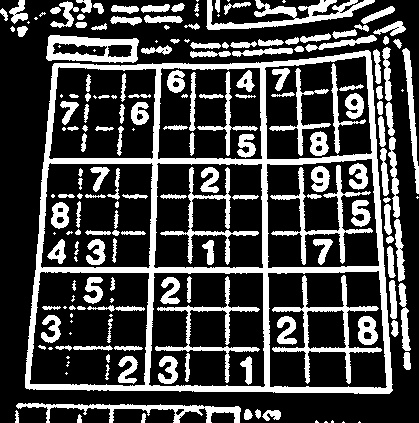
\includegraphics[width=\linewidth] {../../test/threshold/1.jpg}
        \caption{Input image}\label{fig:sht_example:a}
    \end{subfigure}\hfill
    \begin{subfigure}{0.3\textwidth}
        
\includegraphics[width=\linewidth] {../../packages/js-benchmarks/img/seq.png}
        \caption{Accumulator}\label{fig:sht_example:b}
    \end{subfigure}\hfill
    \begin{subfigure}{0.3\textwidth}
        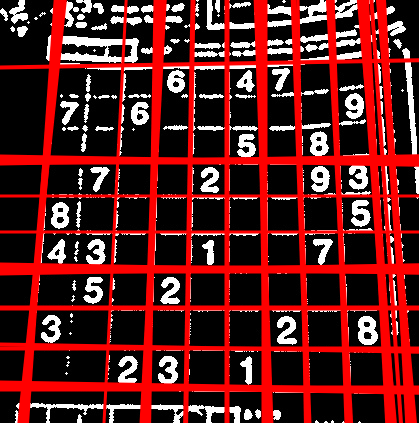
\includegraphics[width=\linewidth] {img/sht_result.png}
        \caption{Detected lines}\label{fig:sht_example:c}
    \end{subfigure}
    \caption{Input image, accumulator and visualized result of sequential SHT algorithm in non-LUT variant ($S_\theta = 1, S_\rho=1$).}\label{fig:sht_example}
\end{figure}

Benchmarks were performed on a platform equipped with Intel\textsuperscript{\tiny\textregistered} Core\textsuperscript{\tiny\texttrademark} i7-12700KF CPU and Nvidia 970 GTX GPU using Ubuntu 20.04.1. The CPU had frequency scaling turned off and due to its hybrid architecture only 4 P-Cores were enabled for a benchmark using \texttt{taskset} utility.

\section{Results and details}\label{sec:results}
In this section, we present execution times for each method depending on angular sampling $S_\theta$ which should result in linear computational complexity. Section \ref{sec:results:sequential} shows times for sequential execution which is then marked as a grey area for comparison. Every chart contains native C++ times. 

\subsection{Sequential}\label{sec:results:sequential}

% MARK: times math
Analyzing benchmark times shown in Figure \ref{plot:sequential} we can see the advantage of Chrome over Firefox being $1.61\times$ faster in the \textit{non-LUT} variant and $2.87\times$ in the \textit{LUT} one. It is worth noticing the optimization in Firefox for the $S_\theta=5$ and subsequent sampling values in the \textit{LUT} variant which could be an object of further research. The performance of server-side environments, Node and Deno, since they are very similar environments, has only insignificant differences, yet still being $~(1.47, 2.06)\times$ slower than Chrome for both variants.



\begin{figure}
    \groupBenchmark{
        \plotBenchmark{cpp_theta_SHT_Simple.csv}{cppColor}{{}}
        \addlegendentry{C++}

        \plotBenchmark{js-sequential_theta_SHT_Simple_node.csv}{nodeColor}{{}}
        \addlegendentry{Node}

        \plotBenchmark{js-sequential_theta_SHT_Simple_deno.csv}{denoColor}{{}}
        \addlegendentry{Deno}

        \plotBenchmark{js-sequential_theta_SHT_Simple_Firefox.csv}{firefoxColor}{{}}
        \addlegendentry{Firefox}

        \plotBenchmark{js-sequential_theta_SHT_Simple_Chrome.csv}{chromeColor}{{}}
        \addlegendentry{Chrome}

    } {
        \plotBenchmark{cpp_theta_SHT_Simple_Lookup.csv}{cppColor}{{}}
        \addlegendentry{C++}

        \plotBenchmark{js-sequential_theta_SHT_Simple_Lookup_node.csv}{nodeColor}{{}}
        \addlegendentry{Node}

        \plotBenchmark{js-sequential_theta_SHT_Simple_Lookup_deno.csv}{denoColor}{{}}
        \addlegendentry{Deno}

        \plotBenchmark{js-sequential_theta_SHT_Simple_Lookup_Firefox.csv}{firefoxColor}{{}}
        \addlegendentry{Firefox}

        \plotBenchmark{js-sequential_theta_SHT_Simple_Lookup_Chrome.csv}{chromeColor}{{}}
        \addlegendentry{Chrome}
    } {
        \plotBenchmark{cpp_theta_CHT_Simple.csv}{cppColor}{{}}
        \addlegendentry{C++}

        \plotBenchmark{js-sequential_theta_CHT_Simple_node.csv}{nodeColor}{{}}
        \addlegendentry{Node}

        \plotBenchmark{js-sequential_theta_CHT_Simple_deno.csv}{denoColor}{{}}
        \addlegendentry{Deno}

        \plotBenchmark{js-sequential_theta_CHT_Simple_Firefox.csv}{firefoxColor}{{}}
        \addlegendentry{Firefox}

        \plotBenchmark{js-sequential_theta_CHT_Simple_Chrome.csv}{chromeColor}{{}}
        \addlegendentry{Chrome}
    }
    [3400][850][14]
    \caption{Wyniki pomiarów czasu wydajności dla wykonania sekwencyjnego SHT i CHT.}
    \label{plot:sequential}
\end{figure}



We detected one-pixel difference in generated accumulator between variants as shown in Figure \ref{fig:diff:seq_lut} (upper right corner). We implemented lookup table for \textit{LUT} variants using \texttt{Float32Array}. JS internally, without optimizations, represents numbers in double-precision and reduced precision of cached values can have a significant impact on detection results.

\begin{figure}
    \begin{subfigure}{0.29\textwidth}
        
\includegraphics[width=\linewidth] {../../packages/js-benchmarks/img/diff_seq_seq_lookup.png}
        \caption{Sequential \textit{LUT}}\label{fig:diff:seq_lut}
    \end{subfigure}\hfill
    \begin{subfigure}{0.29\textwidth}
        
\includegraphics[width=\linewidth] {../../packages/js-benchmarks/img/diff_seq_wasm.png}
        \caption{WASM}\label{fig:diff:wasm}
    \end{subfigure}\hfill
    \begin{subfigure}{0.29\textwidth}
        
\includegraphics[width=\linewidth] {../../packages/js-benchmarks/img/diff_seq_gpu.png}
        \caption{WebGL}\label{fig:diff:gpu}
    \end{subfigure}
    \caption{Normalized absolute accumulator difference from sequential \textit{non-LUT} variant. Note the two-pixel difference in the upper right corner for Sequential \textit{LUT}.}\label{fig:diff}
\end{figure}



\subsection{Node C++ addon}\label{sec:results:cpp-addon}

C++ addon for Node was built using the same shared library as the C++ version. Thus the difference in performance between native C++ and the addon arises mostly from handling data transfer between C++ -- JS boundary since the data needs to be copied and transformed to corresponding C++ structures. Results are shown in Figure \ref{plot:cpu-addon}.



\begin{figure}
    \groupBenchmark{
        \plotBenchmark{cpp-addon_theta_SHT_Simple_node.csv}{nodeColor}{{}}
        \addlegendentry{Node}

        \seqReference
    } {
        \plotBenchmark{cpp-addon_theta_SHT_Simple_Lookup_node.csv}{nodeColor}{{}}
        \addlegendentry{Node}

        \seqReferenceLookup
    }[1600][650]
    \label{plot:gpu}
    \caption{Node C++ addon SHT execution benchmark results.}
\end{figure}

% MARK: times math
Compilation with optimization of trigonometric functions in \textit{non-LUT} variant allowed to gain more performance ($2.24\times$) than compilation of the \textit{LUT} variant ($1.32\times$) relative to their sequential variants. This case allows us to draw a conclusion that if an algorithm has trigonometric functions and output which cannot be cached beforehand, the usage of the C++ addon in Node is beneficial.

\subsection{WebAssembly and asm.js}\label{sec:results:asm-wasm}

Benchmark results for asm.js and WASM were shown on figures \ref{plot:asm} and \ref{plot:wasm} respectively. In our case asm.js - a highly optimizable subset of JS instructions, operating only on numeric types and using heap memory - is actually slower in all environments than sequential execution. We suspect that it is caused by the building process. Webpack adds its own module resolution mechanisms that prevent part of the bundle with asm.js code from being recognized and compiled ahead-of-time. Performance flame chart from Chrome DevTools tools shows a~lack of \texttt{Compile Code} blocks, unlike any other isolated asm.js sample.

WASM on the other hand improves performance for \textit{non-LUT} variant and has no effect on \textit{LUT} variant besides preventing optimization mentioned in section \ref{sec:results:sequential} in Firefox. Again, it is beneficial to use this method if the output of trigonometric functions cannot be cached.

In our C++ implementation we use single precision floating point variables. This results in accumulator differences shown in Figure \ref{fig:diff:wasm} since WASM distinguishes between \texttt{f32} and \texttt{f64} types.



\begin{figure}[ht]
    \groupBenchmark{
        \plotBenchmark{js-asm_theta_SHT_Simple_node.csv}{nodeColor}{{}}
        \addlegendentry{Node}

        \plotBenchmark{js-asm_theta_SHT_Simple_Firefox.csv}{firefoxColor}{{}}
        \addlegendentry{Firefox}

        \plotBenchmark{js-asm_theta_SHT_Simple_Chrome.csv}{chromeColor}{{}}
        \addlegendentry{Chrome}

        \seqReference
    } {
        \plotBenchmark{js-asm_theta_SHT_Simple_Lookup_node.csv}{nodeColor}{{}}
        \addlegendentry{Node}

        \plotBenchmark{js-asm_theta_SHT_Simple_Lookup_Firefox.csv}{firefoxColor}{{}}
        \addlegendentry{Firefox}

        \plotBenchmark{js-asm_theta_SHT_Simple_Lookup_Chrome.csv}{chromeColor}{{}}
        \addlegendentry{Chrome}

        \seqReferenceLookup
    }{
        \plotBenchmark{js-asm_theta_CHT_Simple_node.csv}{nodeColor}{{}}
        \addlegendentry{Node}

        \plotBenchmark{js-asm_theta_CHT_Simple_Firefox.csv}{firefoxColor}{{}}
        \addlegendentry{Firefox}

        \plotBenchmark{js-asm_theta_CHT_Simple_Chrome.csv}{chromeColor}{{}}
        \addlegendentry{Chrome}

        \seqReferenceCircle
    }[9000][2300][25]
    \caption{Wyniki pomiarów czasu wydajności dla wykonania SHT i CHT z wykorzystaniem kompilacji do asm.js.}
    \label{plot:asm}
\end{figure}


\begin{figure}[h]
    \groupBenchmark{
        \plotBenchmark{js-wasm_theta_SHT_Simple_node.csv}{nodeColor}{{}}
        \addlegendentry{Node}

        \plotBenchmark{js-wasm_theta_SHT_Simple_Firefox.csv}{firefoxColor}{{}}
        \addlegendentry{Firefox}

        \plotBenchmark{js-wasm_theta_SHT_Simple_Chrome.csv}{chromeColor}{{}}
        \addlegendentry{Chrome}

        \seqReference
    } {
        \plotBenchmark{js-wasm_theta_SHT_Simple_Lookup_node.csv}{nodeColor}{{}}
        \addlegendentry{Node}

        \plotBenchmark{js-wasm_theta_SHT_Simple_Lookup_Firefox.csv}{firefoxColor}{{}}
        \addlegendentry{Firefox}

        \plotBenchmark{js-wasm_theta_SHT_Simple_Lookup_Chrome.csv}{chromeColor}{{}}
        \addlegendentry{Chrome}

        \seqReferenceLookup
    } {
        \plotBenchmark{js-wasm_theta_CHT_Simple_node.csv}{nodeColor}{{}}
        \addlegendentry{Node}

        \plotBenchmark{js-wasm_theta_CHT_Simple_Firefox.csv}{firefoxColor}{{}}
        \addlegendentry{Firefox}

        \plotBenchmark{js-wasm_theta_CHT_Simple_Chrome.csv}{chromeColor}{{}}
        \addlegendentry{Chrome}

        \seqReferenceCircle
    }[2500][950][15]
    \caption{Wyniki pomiarów czasu wydajności dla wykonania SHT i CHT z wykorzystaniem kompilacji do WASM.}
    \label{plot:wasm}
\end{figure}



\subsection{WebAssembly SIMD}

% MARK: times math
SIMD instructions in WASM are available from Chrome 91 and Firefox 89 for all users. The usage of SIMD instructions can be done implicitly by letting the compiler (commonly LLVM) perform the auto-vectorization process or explicitly by using vector instructions in code. We tested both solutions resulting in no difference from sequential benchmarks for the first one. Because of that, we present only an explicit usage attempt. In benchmarks shown in Figure \ref{plot:wasm_simd_explicit} we can see that the performance difference between Chrome and Firefox decreased compared to sequential execution and Chrome is only $1.16\times$ faster than Firefox. Moreover, Firefox overtakes Node in performance, which was not as prone to SIMD optimization as other environments.

\begin{figure}[h]
    \groupBenchmark{
        \plotBenchmark{js-wasm_simd_explicit_theta_SHT_Simple_node.csv}{nodeColor}{{}}
        \addlegendentry{Node}

        \plotBenchmark{js-wasm_simd_explicit_theta_SHT_Simple_Firefox.csv}{firefoxColor}{{}}
        \addlegendentry{Firefox}

        \plotBenchmark{js-wasm_simd_explicit_theta_SHT_Simple_Chrome.csv}{chromeColor}{{}}
        \addlegendentry{Chrome}

        \seqReference
    } {
        \plotBenchmark{js-wasm_simd_explicit_theta_SHT_Simple_Lookup_node.csv}{nodeColor}{{}}
        \addlegendentry{Node}

        \plotBenchmark{js-wasm_simd_explicit_theta_SHT_Simple_Lookup_Firefox.csv}{firefoxColor}{{}}
        \addlegendentry{Firefox}

        \plotBenchmark{js-wasm_simd_explicit_theta_SHT_Simple_Lookup_Chrome.csv}{chromeColor}{{}}
        \addlegendentry{Chrome}

        \seqReferenceLookup
    }{
        \plotBenchmark{js-wasm_simd_explicit_theta_CHT_Simple_node.csv}{nodeColor}{{}}
        \addlegendentry{Node}

        \plotBenchmark{js-wasm_simd_explicit_theta_CHT_Simple_Firefox.csv}{firefoxColor}{{}}
        \addlegendentry{Firefox}

        \plotBenchmark{js-wasm_simd_explicit_theta_CHT_Simple_Chrome.csv}{chromeColor}{{}}
        \addlegendentry{Chrome}

        \seqReferenceCircle
    }[2200][650][15]
    \caption{Wyniki pomiarów czasu wydajności dla wykonania SHT i CHT z wykorzystaniem kompilacji do WASM z ręczną implementacją instrukcji SIMD.}
    \label{plot:wasm_simd_explicit}
\end{figure}


\subsection{Workers}

All worker benchmarks used concurrency $n=4$. Results are shown in Figure \ref{plot:workers}. Because of the simplified implementation described in section \ref{sec:benchmarking}, precisely the center of the polar coordinate system in image space, the \nth{3} worker is redundant. The \nth{3} vertical quarter of the accumulator will always be empty as shown on example accumulator visualization in Figure \ref{fig:sht_example:b}. This was not optimized in our implementation.


The Table \ref{tab:worker_speedup} shows the speedup and its efficiency for environments and variants. The big difference in speedup efficiency between variants again shows us how demanding calculations of trigonometric functions are. Only the accumulator filling process was parallelized thus the speedup difference between environments is expected since the worker calculations take less time due to the lookup tables.

\begin{wraptable}{r}{6cm}
    \caption{Speedup metrics for worker acceleration method ($S_\theta = 1, p = 4$).}
    \label{tab:worker_speedup}
    \setlength{\tabcolsep}{0.5em}
    \begin{tabular}{lrr}%
        \hline
        Env.        & Speedup & Efficiency              \\
        \hline
        Chrome      & 2.99    & 0.75                    \\
        Firefox     & 2.82    & 0.70                    \\
        Node        & 3.25    & \textcolor{green!70!black}{0.81} \\
        Deno        & 2.70    & \textcolor{red}{0.67}   \\
        Chrome \textit{LUT}  & 1.85    & 0.46                    \\
        Firefox \textit{LUT} & 1.89    & 0.47                    \\
        Node \textit{LUT}    & 1.76    & 0.44                    \\
        Deno \textit{LUT}    & 1.51    & \textcolor{red}{0.38}   \\
        \hline
    \end{tabular}
\end{wraptable}
 
Our implementation can be improved to achieve better performance because the voting process is not parallelized. Even though, the current state of implementation still allows us to compare this method across environments.


We share the accumulator array between workers and it is important to mention that our implementation does not use \texttt{Atomics} since every worker operates on a different part of the array. According to our benchmarks, usage of \texttt{Atomics} tends to slow down performance and was not necessary in this case.



\begin{figure}
    \groupBenchmark{
        \plotBenchmark{js-workers_theta_SHT_Simple_node.csv}{nodeColor}{{}}
        \addlegendentry{Node}

        \plotBenchmark{js-workers_theta_SHT_Simple_deno.csv}{denoColor}{{}}
        \addlegendentry{Deno}

        \plotBenchmark{js-workers_theta_SHT_Simple_Firefox.csv}{firefoxColor}{{}}
        \addlegendentry{Firefox}

        \plotBenchmark{js-workers_theta_SHT_Simple_Chrome.csv}{chromeColor}{{}}
        \addlegendentry{Chrome}

        \seqReference
    } {
        \plotBenchmark{js-workers_theta_SHT_Simple_Lookup_node.csv}{nodeColor}{{}}
        \addlegendentry{Node}

        \plotBenchmark{js-workers_theta_SHT_Simple_Lookup_deno.csv}{denoColor}{{}}
        \addlegendentry{Deno}

        \plotBenchmark{js-workers_theta_SHT_Simple_Lookup_Firefox.csv}{firefoxColor}{{}}
        \addlegendentry{Firefox}

        \plotBenchmark{js-workers_theta_SHT_Simple_Lookup_Chrome.csv}{chromeColor}{{}}
        \addlegendentry{Chrome}

        \seqReferenceLookup
    }[1700][500]
    \label{plot:workers}
    \caption{Workers SHT execution benchmark results with concurrency $n=4$. Gray area shows sequential JavaScript execution performance range. Non-LUT variant performs better than sequential execution. On the other hand the LUT one has gained only small increase in performance.}
    % TODO: speedup math
\end{figure}


\subsection{WebGL}

Our last acceleration method uses a GPGPU to fill the accumulator array. With help of the WebGL and the gpu.js library, we implemented kernel functions calculating every pixel separately. It is the only possible solution since the WebGL pipeline does not provide shared memory. This results in a bigger accumulator difference shown in Figure \ref{fig:diff:gpu}. First of all, the pipeline provides only single-precision operations. Secondly, for every accumulator value - pair ($\theta$, $\rho$), we had to sum image pixels laying on a possible line. This operation is prone to rounding errors. Additionally, the minification of the output bundle provided by Webpack was interfering with the way the gpu.js library transpiles code to a GLSL language. We had to construct the function from string to prevent minification of the kernel function -- \lstinline[language=JavaScript]|new Function('return function (testImage) {...}')()|.

This method tends to have the biggest result variance which comes directly from communication between CPU and GPU. It has also the biggest cold start times since the kernel has to be compiled by an environment on the first run. There is no big difference between both variants because in the \textit{non-LUT} variant each thread on the GPU has to calculate $sin$ and $cos$ functions once which is not a significant overhead.


\begin{figure}
    \groupBenchmark{
        %\plotBenchmark{js-gpu_theta_SHT_Simple_node.csv}{nodeColor}{{}}
        %\addlegendentry{Node}

        %\plotBenchmark{js-gpu_theta_SHT_Simple_deno.csv}{denoColor}{{}}
        %\addlegendentry{Deno}

        \plotBenchmark{js-gpu_theta_SHT_Simple_Firefox.csv}{firefoxColor}{{}}
        \addlegendentry{Firefox 95}

        \plotBenchmark{js-gpu_theta_SHT_Simple_Chrome.csv}{chromeColor}{{}}
        \addlegendentry{Chrome 97}

        \seqReference
    } {
        %\plotBenchmark{js-gpu_theta_SHT_Simple_Lookup_node.csv}{nodeColor}{{}}
        %\addlegendentry{Node}

        %\plotBenchmark{js-gpu_theta_SHT_Simple_Lookup_deno.csv}{denoColor}{{}}
        %\addlegendentry{Deno}

        \plotBenchmark{js-gpu_theta_SHT_Simple_Lookup_Firefox.csv}{firefoxColor}{{}}
        \addlegendentry{Firefox 95}

        \plotBenchmark{js-gpu_theta_SHT_Simple_Lookup_Chrome.csv}{chromeColor}{{}}
        \addlegendentry{Chrome 97}

        \seqReferenceLookup
    }[550][200]
    \label{plot:gpu}
    \caption{WebGL SHT execution benchmark results. Gray area shows sequential JavaScript execution performance range.}
\end{figure}


\section{Conclusions}\label{sec:conclusions}
We performed various benchmarks of the same algorithm in Chrome, Firefox, Node and Deno environments (Tab. \ref{tab:versions}). In each one we tested available and popular acceleration methods including native addon, WASM alone, WASM with SIMD instructions, multi-threading with workers and GPGPU using \mbox{WebGL} graphics pipeline. We did not test every method on every environment because of being unavailable, unstable, under a flag or basing on non-C++ codebase (Tab. \ref{tab:implemented}). Summarized results for the same problem size are shown in table \ref{tab:envs}.
In every benchmark Chrome appears as the fastest environment with Firefox being $2.24\times$, Node $1.49\times$ and Deno $1.59\times$ slower in general. As expected, without involving parallel execution, the Node C++ native addon brings the best results across all environments. Server-side environments preformed similarly with slight predominance of Node over Deno.

According to our results, the performance of \textit{LUT} variant was always better than its \textit{non-LUT} counterpart. Trigonometric functions are demanding but our study shows that using native addon or compiling code to WASM can prevent significant performance loss, especially in the Firefox environment. We can see that Firefox is not able to optimize code as well as other environments, where using vector instructions explicitly actually lowers performance, increasing it in Firefox.
When using lookup tables results may be different. Looking at Chrome performance of all WASM methods with \textit{LUT} variant we can see that performance is roughly the same with the sequential. Data exchanged between JS and WASM must be transformed and copied, which takes time, so it is not safe to assume performance benefit with intensive memory input and output when adopting WASM.
We also identified problem with asm.js. which wasn't compiled ahead-of-time. We suspect that the bundling system and minification process prevented environments from recognizing asm.js specific code. 

To sum up, all environments serve similar cases but differ in terms of the performance of various acceleration methods. It is important to analyze which method best suits our needs depending on requirements. 
%We hope that this analysis will help to find the most efficient way to speed up execution making JavaScript a more robust environment for CPU-intensive computations. 
With all this, it is important to remember that no acceleration method can increase the performance of an algorithm like improvement of the computational complexity of the algorithm itself.

\newcommand{\comma}{, }
\begin{table}
    \label{tab:envs}
    \caption{Comparison of implemented methods in analyzed environments. The general comparison was done using Chrome as a reference point and geometric mean for times comparable with Chrome.}

    \begin{tabularx}{\linewidth}{X r r r r}%
        \hline
                                 & \multicolumn{4}{c}{\bfseries Execution time[ms]}                                                             \\
        \bfseries Method         & \bfseries Chrome                                 & \bfseries Firefox     & \bfseries Node  & \bfseries Deno

        \csvreader[
            head to column names,
            before first line=                                                                                                                  \\\hline,
            late after line=                                                                                                                    \\,
            late after last line=                                                                                                               \\\hline
        ]{../../benchmark/environments/envs.csv}{}% use head of csv as column names
        {
        \name\                   & \chrome\ (\chromeF)                              & \firefox\ (\firefoxF) & \node\ (\nodeF) & \deno\ (\denoF)
        }% specify your coloumns here 
        \bfseries Geometric mean &
        \csvreader[
            head to column names,
            late after last line=                                                                                                               \\\hline

        ]{../../benchmark/environments/geoMeans.csv}{}% use head of csv as column names
        {
        (\chrome)                & (\firefox)                                       & (\node)               & (\deno)
        }% specify your coloumns here 
    \end{tabularx}

\end{table}


% TODO: identified interesting aspects

% TODO: further research

% TODO: state of multi-environment numerical computing in JS


\clearpage
 
\bibliographystyle{splncs04}
\bibliography{bibliography}

\end{document}
